\documentclass[class=book, crop=false, oneside, 12pt]{standalone}
\usepackage{standalone}
\usepackage{amsmath}
\usepackage{../../style}
\graphicspath{{./assets/images/}}

% arara: pdflatex: { synctex: yes, shell: yes }
% arara: latexmk: { clean: partial }
\begin{document}

\chapter{Gas ideali e reali}

\section{Leggi di gas, equazioni di stato dei gas ideali}

Un gas è un fluido con le seguenti caratteristiche:
\begin{enumerate}
    \item non ha forma né volume proprio, occupa pertanto tutto il volume a disposizione, per esempio quello del recipiente che lo contiene; 
    \item è comprimibile facilmente, con conseguenti variazioni notevoli di volume, densità e pressione.
\end{enumerate}

Considerata una certa quantità di gas, le variabili termodinamiche più appropriate per descrivere lo stato termodinamico del gas e le eventuali trasformazioni sono la pressione \(p\), il volume \(V\) e la temperatura \(T\).

Consideriamo il gas racchiuso dentro un contenitore di volume \(V\), con un valore della pressione eguale in tutti i punti, se \(V\) non è molto grande. 
Quando il volume del contenitore cambia, come può avvenire se una parte dello stesso è mobile, si realizza uno scambio di lavoro con l'ambiente esterno; inoltre, a seconda del tipo di pareti del contenitore, diatermiche o adiabatiche, è possibile o viene impedito lo scambio di calore con l'ambiente. 
Il gas può dunque compiere trasformazioni in cui scambia soltanto lavoro o calore con l'ambiente, oppure entrambi; in ogni caso il bilancio energetico è regolato dal primo principio della termodinamica.

\subsection{Legge isoterma di Boyle}

Si abbia un gas in equilibrio termodinamico ad una certa pressione entro un dato volume e a temperatura \(T\): se si fanno variare i valori della pressione e del volume, mantenendo costante la temperatura, si trova che in tutti i possibili stati di equilibrio isotermi vale la relazione:
\begin{equation} \label{legge_boyle}
    pV = costante
\end{equation}
\emph{a temperatura costante la pressione è inversamente proporzionale al volume}.

Una trasformazione isoterma tra due stati di equilibrio di un gas si può realizzare, ad esempio, se il contenitore, a pareti diatermiche, è  mantenuto in contatto termico con una sorgente di calore alla temperatura \(T\) e la parete mobile si muove a seguito di una differenza infinitesima di pressione tra gas e ambiente esterno. 
Si hanno condizioni di equilibrio meccanico e termico e possiamo assumere che durante la trasformazione la temperatura sia costante e la pressione del gas sempre eguale a quella esterna.

In un sistema di coordinate cartesiane ortogonali nel piano, con il volume sull'asse delle ascisse e la pressione sull'asse delle ordinate, il luogo dei punti che rappresentano gli stati di equilibrio di un gas a una data temperatura è costituito da un ramo di iperbole.
Per ogni temperatura si ha una diversa iperbole e le curve così ottenute si chiamano "le isoterme del gas ideale". 

\subsection{Legge isobara di Volta-Gay Lussac}

Se la pressione di un gas durante una trasformazione resta costante, si parla di trasformazione isobara; si verifica che in condizioni isobare il volume varia linearmente con la temperatura:
\begin{equation}
    V = V_0 (1 + \alpha t)
\end{equation}
la temperatura è espressa in gradi Celsius, \(V_0\) è il volume occupato dal gas per \(t=0\) e \(\alpha\) è una costante che varia poco al variare del tipo di gas, detta \emph{coefficiente di dilatazione termica}.

Per provare la validità della legge isobara di Volta-Gay Lussac si può mettere il gas in equilibrio termico con diverse sorgenti di calore, mantenendo sempre l'equilibrio meccanico con l'ambiente (pressione interna eguale alla pressione esterna costante) e ogni volta misurare il volume del contenitore, che ha una parete mobile. 
La trasformazione isobara, nel piano \(( p, V )\) già considerato, è rappresentata da un segmento di retta parallelo all'asse dei volumi.

\subsection{Legge isocora di Volta-Gay Lussac}

Se invece si mantiene costante il volume di un gas la pressione risulta funzione lineare della temperatura:
\begin{equation}
    p = p_0 (1 + \beta t)
\end{equation}
Anche ora la temperatura è espressa in gradi Celsius; \(p_0\) è la pressione del gas per \(t = 0\) e \(\beta\) una costante, praticamente indipendente dal tipo di gas.

Una trasformazione a volume costante si dice isocora; nel piano \(( p, V )\) essa è rappresentata da un segmento di retta parallelo all'asse delle pressioni.

La verifica della legge isocora di Volta-Gay Lussac si può eseguire utilizzando il solito contenitore, mantenendo bloccata la parete mobile e misurando la pressione in diversi stati di equilibrio, con il gas in contatto termico con diverse sorgenti di calore.

Ricordiamo quanto detto all'inizio e cioè che il comportamento dei diversi gas è in accordo con le leggi precedenti quanto più ci si avvicina alle condizioni di gas ideale (bassa pressione e alta temperatura). 
Così facendo si osserva anche che le costanti \(\alpha\) e \(\beta\) assumono lo stesso valore per tutti i gas: 
\begin{equation*}
    \alpha = \beta = \frac{1}{273.15} ^{\circ} C^{-1}
\end{equation*}

Posso quindi riscrivere le leggi 
\begin{equation}
    V = V_0 \alpha (\frac{1}{\alpha} + t) = V_0 \alpha T
\end{equation}
\begin{equation}
    p = p_0 \alpha (\frac{1}{\alpha} + t) = p_0 \alpha T
\end{equation}
dove con \(T = \frac{1}{\alpha} + t = 272.15 + t \) è indicata la temperatura misurata in Kelvin.

\subsection{Legge di Avogadro}

La legge di Avogadro stabilisce che \emph{volumi eguali di gas diversi, alla stessa temperatura e pressione, contengono lo stesso numero di molecole}.
Essa si riferisce a gas che abbiano un comportamento ideale e quindi obbediscano alle leggi precedentemente enunciate.

Se si considera una massa \(M\) eguale ad \(A\) grammi di gas, quantità che si chiama mole, il numero di Avogadro vale:
\begin{equation*}
    N_A = 6.0221 \cdot 10^{23} molecole/mole
\end{equation*}

Dalla legge di Avogadro discende la definizione della settima unità fondamentale, quella della quantità di materia. 
Si chiama mole una quantità di materia che contiene tante entità elementari quanti sono gli atomi contenuti in \(0.012 kg\) dell'isotopo \(^{12} C\) del carbonio.

Come conseguenza della legge di Avogadro \emph{una mole di qualsiasi gas, a una data temperatura e pressione, occupa sempre lo stesso volume}.\newline
Si trova che se la pressione è quella atmosferica (\( p_0 = 101325 Pa\)) e la temperatura è \(T_0 = 273.15 K = 0 ^{\circ} C \), tale volume vale \(V_m\)viene indicato col nome di \emph{volume molare}. 
Pertanto \(n\) moli occupano un volume pari a \(n V_m\) e in particolare una chilomole occupa \(22.414 m^3\), nelle dette condizioni di pressione e temperatura. 

\subsection{Equazione di stato del gas ideale}

Se consideriamo \(n\) moli di un gas alla pressione atmosferica \(p_0\) e alla temperatura \(T_0 = 273.15 K\), esse occupano, come abbiamo appena detto, il volume \(V_0 = n V\).

Mantenendo costante il volume e portando la temperatura al valore \(T\)
\begin{equation*}
    p_T = p_0 \alpha T
\end{equation*} 

Moltiplicando per \(V_0\) si ha
\begin{equation*}
    p_T V_0 = p_0 V_0 \alpha T = p_0 V_T
\end{equation*}
\(V_0\) e \(p_T\) sono le coordinate termodinamiche in un particolare stato di equilibrio alla temperatura \(T\), 
come lo sono \(p_0\) e \(V_T\) per un altro stato, sempre alla temperatura \(T\).

Otteniamo dunque:
\begin{equation*}
    pV = p_0 V_0 \alpha T = n p_0 V_m \alpha T
\end{equation*}

Il prodotto \(p_0 V_m \alpha\) è una costante universale, che ha lo stesso valore per tutti i gas, e quindi: 

\subsubsection*{Legge di stato del gas ideale}

\begin{equation} \label{eq_stato_gas_ideale}
    p V = n R T
\end{equation}
con
\begin{equation*}
    R = p_0 V_m \alpha = 1.01325 \cdot 10^5 \cdot 0.022414 \cdot \frac{1}{273.15} = 8.314 \frac{J}{mole K}
\end{equation*}

Definiamo, sulla base delle tre leggi elementari e della legge di Avogadro, come \emph{gas ideale un sistema le cui coordinate termodinamiche in uno stato di equilibrio obbediscono alla (\(\ref{eq_stato_gas_ideale}\)), detta equazione di stato di un gas ideale.}

L'equazione di stato contiene le leggi precedenti: infatti basta mantenere costante \(T\), \(p\) o \(V\) in (\ref{eq_stato_gas_ideale})  e si ottengono le tre leggi isoterma, isobara o isocora. 
Anche la legge di Avogadro è contenuta in (\ref{eq_stato_gas_ideale}), se \(R\) è una costante universale.

Ricordando che \(n = \frac{N}{N_A}\), con \(N\) numero di molecole del gas, abbiamo 
\begin{equation}
    p V = \frac{N}{N_A} R T = N k_b T
\end{equation}
la costante universale
\begin{equation}
    k_b = \frac{R}{N_A} = \frac{8.314}{6.0221 \cdot 10^23} = 1.3807 \cdot 10^{-23} \udm{J/K}
\end{equation}
è detta costante di Boltzmann.

L'equazione di stato dei gas ideali esprime un comportamento limite, al quale si avvicinano i gas reali quanto più lontana è la loro temperatura da \(T = 0\) e quanto più bassa è la loro pressione ovvero la loro densità, cioè quanto più sono caldi e rarefatti. 
In queste condizioni le differenze di comportamento dei diversi gas praticamente scompaiono e tutti seguono approssimativamente (\ref{eq_stato_gas_ideale}).

\section{Trasformazioni di un gas, lavoro}

Consideriamo due stati di equilibrio \(A\) e \(B\) di un sistema formato da \(n\) moli di gas ideale. 
Noti i valori della pressione e del volume, dall'equazione di stato (\ref{eq_stato_gas_ideale}) si ricavano i valori della temperatura:
\begin{equation*}
    T_A = \frac{p_A V_A}{n R}
\end{equation*}
\begin{equation*}
    T_B = \frac{p_B V_B}{n R}
\end{equation*}

Una trasformazione che porti il gas dallo stato \(A\) allo stato \(B\) può svolgersi attraverso stati di equilibrio termodinamico ed è rappresentabile nel piano (\(p , V\)) da una curva continua.
Se invece la trasformazione ha luogo attraverso stati di non equilibrio si usa una rappresentazione simbolica a tratti per indicare che si ignorano i valori delle coordinate durante il processo.

La trasformazione attraverso stati di non equilibrio può realizzarsi in conseguenza di un processo di espansione o compressione rapida, per cui non sussiste né equilibrio meccanico né termico, o per effetto di una espansione o compressione lenta con una differenza di pressione finita così che, pur potendoci essere equilibrio termico, non c'è equilibrio meccanico, oppure a seguito di contatto termico con differenza finita di temperatura.

Quando un gas si espande o viene compresso avviene uno scambio di lavoro che in termini infinitesimi si può scrivere in generale \( d W = p d V\). 
In una trasformazione finita dallo stato \(A\) allo stato \(B\) si avrebbe
\begin{equation} \label{trasf_finita_a_b}
    W = \int_A^B p(V) d V
\end{equation}
però bisogna fare attenzione perché questa espressione esplicita del lavoro è valida sostanzialmente in due sole situazioni: 
\begin{enumerate}
    \item \emph{se la trasformazione è reversibile} e pertanto si può calcolare l'integrale, dato che la pressione è determinata in ogni stato intermedio \(p = p_{gas} = p_{amb}\);
    \item \emph{se è nota la pressione esterna} che, per esempio, è costante, caso tipico di quando il processo avviene sotto la pressione atmosferica; in questa situazione, anche se la trasformazione non è reversibile, il lavoro è calcolabile ed è dato da
    \begin{equation*}
        W = p_{amb} (V_B - V_A)
    \end{equation*}
    In tutti gli altri casi in cui la pressione non è nota non si può applicare la (\ref{trasf_finita_a_b}).
\end{enumerate}

Ad ogni modo, se la trasformazione è isocora (\(V =\) costante, \(\Delta V = 0\)), il lavoro è sempre nullo; se il gas si espande il volume finale \(V_B\) è maggiore del volume iniziale e il gas compie un lavoro sull'ambiente che secondo la convenzione adottata è positivo; 
se il gas viene compresso, \(V_B < V_A\) e il gas subisce un lavoro (negativo), compiuto dall'ambiente.

Il lavoro, se si può utilizzare (\ref{trasf_finita_a_b}), ha un semplice significato geometrico nel piano (\(p,V\)). 
Nel caso di una trasformazione che passa attraverso stati di equilibrio ed è quindi rappresentabile con una curva continua, la curva \(p = p (V)\) nel piano (\(p, V\)), il lavoro, in accordo con il significato geometrico dell'operazione di integrazione, è pari all'area compresa tra la curva e l'asse dei volumi. 

\section{Energia interna del gas ideale}

La dipendenza dell'energia interna di un gas ideale dalle coordinate termodinamiche è stata ricavata analizzando il risultato dell'\emph{esperienza sull'espansione libera, eseguita da Joule}. 

\begin{figure}[h]
    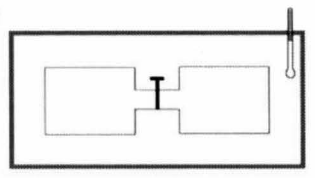
\includegraphics[scale=0.4]{espansione_libera.png}
    \centering
    \caption{}
\end{figure}

In un contenitore con pareti rigide e diatermiche, diviso in due parti eguali separate da un rubinetto, si trova un gas nella parte sinistra, mentre nella parte destra è stata realizzata una condizione di vuoto. 
Il contenitore è immerso in un calorimetro e la temperatura di equilibrio è \(T\). 
Si apre il rubinetto e si lascia espandere il gas in tutto il volume a disposizione. 
L'espansione è chiamata libera perché non ci sono forze esterne che agiscono sul gas.
Sperimentalmente si osserva che, comunque si operi, aprendo lentamente o rapidamente il rubinetto, con gas inizialmente ad alta o bassa pressione, la temperatura del liquido calorimetrico alla fine del processo è sempre pari a \(T\), temperatura iniziale di equilibrio.

Il gas quindi non scambia calore con il calorimetro, \(Q = 0\). 
Esso inoltre non scambia lavoro con l'esterno (le pareti del contenitore sono rigide) e pertanto \(W = 0\). 
Dal primo principio segue \(\Delta V = Q - W = 0\): \emph{nell'espansione libera l'energia interna di un gas ideale non varia}. 
Possiamo allora giungere alla seguente conclusione: poiché nel processo la temperatura del gas non cambia, mentre variano pressione e volume (in accordo con \ref{legge_boyle} perché la trasformazione è isoterma, cioè \(p_{in} V_{in} = p_{fin} V_{fin}\)), l'energia interna deve essere funzione soltanto della temperatura. 

\begin{figure}[h]
    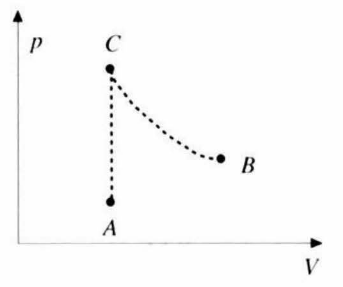
\includegraphics[scale=0.4]{ACB.png}
    \centering
    \caption{}
\end{figure}

Per determinare l'espressione esplicita della funzione \(U(T)\) consideriamo due generici stati di equilibrio \(A\) e \(B\): \(\Delta U = U_B - U_A\) deve essere la stessa, qualsiasi trasformazione si scelga, essendo \(U\) una funzione di stato.
Se scegliamo, in particolare, una trasformazione \(A C\) isocora e una \(C B\) isoterma, si ha:
\begin{equation*}
    \Delta U = U_B - U_A = U_B - U_C + U_C - U_A = U_C - U_A
\end{equation*}
in quanto \(U_B = U_C\) essendo gli stati \(B\) e \(C\) alla stessa temperatura ed \(U\) funzione sole della temperatura.

Applichiamo ora il primo principio alla trasformazione isocora: dato che \(W = 0, \Delta U = Q\), dove \(Q\) è il calore scambiato in condizioni isocore. 
Pertanto 
\begin{equation}
    \Delta U = U_B - U_A = n c_v (T_B - T_A) = n c_v \Delta T 
\end{equation}
\begin{equation}
    \Delta U = U_B - U_A = n \int_{T_A}^{T_B} c_v d T
\end{equation}
a seconda che il calore specifico a volume costante sia indipendente dalla temperatura oppure no. 
Per trasformazioni infinitesime
\begin{equation}
    d U = n c_v d T
\end{equation}
da cui si ricava
\begin{equation}
    c_v = \frac{1}{n} \frac{d U}{d T}
\end{equation}

Poiché l'energia interna è funzione soltanto della temperatura, anche il calore specifico a volume costante di un gas ideale dipende solo dalla temperatura, potendo essere, in particolare, costante.
Si può quindi scrivere in maniera esplicita il primo principio, per quel che riguarda le trasformazioni ideali:
\begin{equation} \label{primo_principio_trasf_ideali}
    d Q = n c_v d T + d W \implies Q = n \int_{T_A}^{T_B} c_v d T + W
\end{equation}
\begin{equation}
    Q = n c_v \Delta T + d W \ \text{ se } \ c_v = cost
\end{equation}

Se la trasformazione è reversibile, le equazioni precedenti diventano:
\begin{equation}
    d Q = n c_v d T + d p V \implies Q = n \int_{T_A}^{T_B} c_v d T + \int_{V_A}^{V_B} p d V
\end{equation}
\begin{equation}
    Q = n c_v \Delta T + \int_{V_A}^{V_B} p d V \ \text{ se } \ c_v = cost
\end{equation}

\subsection{Relazione di Mayer}

In una trasformazione isobara infinitesima \(d Q = n c_p d T\) e \(d W = p d V\)
\begin{equation*}
    n c_p d T = n c_v d T + p d V
\end{equation*}
Differenziando l'equazione di stato dei gas ideali \(p_V = n R T\) si ha
\begin{equation*}
    p d V + V d p = n R d T
\end{equation*}
in una trasformazione isobara \(d p = 0\) e quindi \(p d V = n R d T\). Pertanto
\begin{equation*}
    n c_p d T = n c_v d T + n R d T
\end{equation*}
semplificando si ottiene la relazione di Mayer
\begin{equation}
    c_p - c_v = R
\end{equation}

Di conseguenza in un gas ideale anche \(c_p\) è funzione soltanto della temperatura potendo in particolare essere costante.

Il rapporto tra calori specifici
\begin{equation}
    \gamma = \frac{c_p}{c_V}
\end{equation}
risulta in un gas ideale sempre maggiore di 1 ed è funzione soltanto della temperatura o, in particolare, costante. 

Sperimentalmente si trovano per i calori specifici dei gas ideali questi risultati:
\begin{enumerate}
    \item i gas ideali monoatomici hanno \(c_V\) costante e pari a \(\frac{3}{2} R\)
    \item alcuni gas ideali biatomici hanno \(c_V\) costante e pari a \(\frac{5}{2} R\)
\end{enumerate}

\section{Studio di alcune trasformazioni}

\begin{figure}[h]
    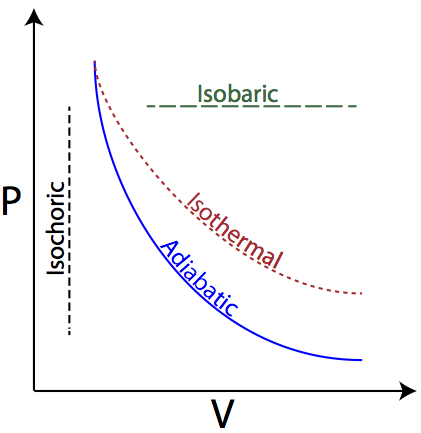
\includegraphics[scale=0.4]{PV_diagram.png}
    \centering
    \caption{}
\end{figure}

\subsection{Trasformazioni adiabatiche}

Il gas è racchiuso dentro un contenitore con pareti adiabatiche e quindi può scambiare solo lavoro, per esempio in conseguenza del fatto che una parete è mobile. 
Dal primo principio si ha
\begin{equation*}
    W_{AB} = - \Delta U = - n c_v (T_B -T_A)
\end{equation*}
se la trasformazione avviene tra i due stati di equilibrio \(A\) iniziale e \(B\) finale. 

Se si ha un'espansione adiabatica il lavoro \(W_{AB}\) è positivo e quindi \(\Delta U\) è negativa e \(T_B\) è minore di \(T_A\): il gas si raffredda; se invece si ha una compressione adiabatica, \(W_{AB}<0, \Delta U > 0 , T_B > T_A\), il gas si riscalda. 
Queste variazioni di temperatura sono comunemente sperimentate nelle variazioni rapide di volume di un gas.

Se invece la trasformazione è \emph{adiabatica reversibile}, l'espressione infinitesima del primo principio diviene
\begin{equation*}
    d U + d W = n c_v d T + p d V = 0
\end{equation*}
in quanto possiamo esprimere il lavoro in funzione delle coordinate termodinamiche, appunto perché la trasformazione è reversibile.

Per questa stessa ragione si può utilizzare l'equazione di stato in qualsiasi stato intermedio per esprimere la pressione come \(p = \frac{n R T}{V}\) e si ottiene
\begin{equation*}
    n c_V d T + \frac{n R T}{V} d V = 0
\end{equation*}

Se pariamo le variabili e utilizziamo la relazione di Mayer
\begin{equation*}
    \frac{c_p -c_V}{c_V} \frac{d V}{V} = - \frac{d T}{T} \implies (\gamma - 1) \frac{d V}{V} = - \frac{d T}{T}
\end{equation*}
Questa equazione differenzia e rappresenta la condizione a cui obbediscono le coordinate degli stati di un gas ideale collegati da una trasformazione adiabatica reversibile.

\begin{equation*}
    (\gamma - 1) \ln \frac{V_{B}}{V_A} = \ln \frac{T_A}{T_B} \implies \ln \left(\frac{V_B}{V_A}\right)^{\gamma - 1 } = \ln \frac{T_A}{T_B}
\end{equation*}
L'eguaglianza tra i logaritmi comporta l'eguaglianza tra gli argomenti, per cui
\begin{equation*}
    T_A V_A^{\gamma - 1} = T_B V_B^{\gamma - 1}
\end{equation*}
espressione che dà la relazione tra le coordinate termodinamiche del gas durante una trasformazione adiabatica reversibile. 

Tramite l'equazione di stato si può trasformare la relazione tra \(T\) e \(V\) in una tra \(p\) e \(V\) o tra \(p\) e \(T\) e in conclusione si hanno tre espressioni equivalenti:
\begin{equation}
    T V^{\gamma - 1 } = costante \ , \ pV^{\gamma} = costante \ , \ T p^{\frac{1 - \gamma}{\gamma}}
\end{equation}

Le (\ref{primo_principio_trasf_ideali}) sono un esempio di quando si possono esprimere i termini del primo principio della dinamica in funzione delle coordinate termodinamiche, ottenendo una relazione tra queste che rappresenta l'equazione della trasformazione.
Esse si chiamano infatti le \emph{equazioni di una trasformazione adiabatica reversibile di un gas ideale}.

In particolare utilizziamo l'equazione \(p V^{\gamma} = costante\) per rappresentare a trasformazione nel piano di Clapeyron. 
Rispetto alla curva isoterma \(p V = costante\), passante per esempio per il punto rappresentativo dello stato \(A\), la curva adiabatica ha un andamento simile però con pendenza maggiore perché \(y\) è sempre maggiore di 1:  si conferma che \(T_B < T_A\).

Una trasformazione adiabatica reversibile costituisce un caso limite, in quanto per essere reversibile dovrebbe svolgersi molto lentamente, ma ciò introduce difficoltà per mantenere l'adiabaticità. 
Le trasformazioni reali sono irreversibili, in particolare possiamo considerare adiabatica irreversibile una trasformazione che comporta una variazione rapida di volume, così che non ci sia tempo per scambi di calore. 

L'espansione libera di Joule è un altro caso di \emph{trasformazione adiabatica irreversibile}.

\subsection{Trasformazione isoterma}

Nel caso di una trasformazione isoterma si considera il gas racchiuso in un recipiente che è in contatto termico con una sorgente di calore alla temperatura \(T\). 
Durante la trasformazione la temperatura del gas resta costante al valore \(T\) e abbiamo
\begin{equation*}
    \Delta U = 0 \ , \ Q = W \ , \ p_A V_A = p_B V_B
\end{equation*}

Se la trasformazione è un espansione isoterma \(W_{AB}>0\) e quindi \(Q_{AB}>0\): il gas compie lavoro e assorbe calore. 
Se invece la trasformazione è una compressione isoterma \(W_{AB} < 0 \) e \(Q_{AB} < 0\): il gas subisce lavoro e cede calore.

Qualora la trasformazione sia isoterma reversibile dalla legge dei gas ideali e dal lavoro in una trasformazione finita si ha
\begin{equation}
    W_{AB} = \int_A^B p d V = \int_A^B \frac{n R T}{V} d V = n R T \int_A^B \frac{d V}{V} = n R T \ln \frac{V_{B}}{V_{A}} 
\end{equation}
e questa è anche l'espressione esplicita del calore scambiato.

Si noti che è sempre \(Q \neq 0\): una trasformazione isoterma reversibile comporta sempre uno scambio di calore, a meno che non sia \(T = 0\), condizione che non è mai raggiungibile. 

Una particolare trasformazione isoterma irreversibile è l'espansione libera di Joule. 
Tale trasformazione è insieme adiabatica e isoterma: ciò è possibile solo perché la trasformazione è irreversibile; per una reversibile i due fatti sono ben distinti ed è impossibile che una trasformazione isoterma sia anche adiabatica.

\subsection{Trasformazioni isocore}

Il gas è contenuto in un recipiente diatermico di volume fisso: \(V = costante\) e \(W = 0\); il gas può scambiare solo calore e questo è eguale, per il primo principio, alla variazione dell'energia interna:
\begin{equation*}
    Q = \Delta U = m c_v (T_B - T_A) \ \  c_v = costante
\end{equation*}

Essendo il volume costante dell'equazione di stato:
\begin{equation*}
    \frac{p_A}{T_A} = \frac{p_B}{T_B} \implies \frac{p_A}{p_B} = \frac{T_A}{T_B}
\end{equation*}
Se si cede calore al gas, la sua pressione e la sua temperatura aumentano, mentre se si assorbe calore dal gas pressione e temperatura diminuiscono.

\subsection{Trasformazioni isobare}

Il gas è contenuto ora in un recipiente diatermico con una parete mobile su cui agisce una pressione esterna costante \(p\).
Dall'equazione di stato o dalle leggi di Gay-Lussac abbiamo che in una trasformazione isobara:
\begin{equation*}
    \frac{v_A}{T_A} = \frac{v_B}{T_B} \implies \frac{v_A}{v_B} = \frac{T_A}{T_B}
\end{equation*}

Il gas può scambiare sia calore che lavoro, dati da 
\begin{equation*}
    Q = n c_p \left(T_B - T_A\right)
\end{equation*}
\begin{equation*}
    W = p (V_B - V_A) = p \left(\frac{n R T_B}{p} - \frac{n R T_A}{p}\right) = n R \left(T_B - T_A\right) 
\end{equation*}
e deve essere sempre \(Q - W = \Delta U = n c_v (T_B - T_A)\).

Se si cede calore al gas, il suo volume e la sua temperatura aumentano e il gas compie lavoro; se si assorbe calore dal gas, volume e temperatura diminuiscono, il gas subisce lavoro.

Una trasformazione isobara si compie mettendo il gas, a temperatura \(T_A\), in contatto termico con una sorgente di calore a temperatura \(T_B\); non essendoci equilibrio termico la trasformazione è irreversibile. 
Invece, per avere una trasformazione reversibile bisogna disporre di una serie infinita di sorgenti, come descritto per le trasformazioni isocore. 

\subsection{Trasformazioni generiche}

Per una trasformazione diversa da quelle precedenti possiamo utilizzare il primo principio nella forma:
\begin{equation}
    d Q = d U + d W = n c_v d T + d W
\end{equation}
È necessario poi esaminare attentamente le condizioni termodinamiche che regolano la trasformazione, per stabilire se essa sia reversibile o irreversibile.

Se è reversibile possiamo utilizzare l'equazione di stato \(p V= n R T\) per il lavoro l'espressione \(d W = p d V \). 
Si tenga presente che per il lavoro conviene verificare se può essere calcolato direttamente per via geometrica, cioè tramite l'area sotto la curva che rappresenta la trasformazione nel piano (\(p , V\)).

\section{Trasformazioni cicliche}

Una trasformazione ciclica o ciclo è una trasformazione in cui lo stato finale coincide con lo stato iniziale. 
Il primo principio ci dice che il calore scambiato è eguale al lavoro scambiato.

Se durante il ciclo viene \emph{prodotto lavoro} (\(W > 0 \)), \emph{assorbendo calore} da un opportuno numero di sorgenti, tale \emph{ciclo} è detto \emph{termico}. 
Il dispositivo che opera è indicato come \emph{macchina termica}. 
Se invece il ciclo è tale che venga \emph{richiesto lavoro esterno} (\(W < 0\)), \emph{estraendo calore} da una o più sorgenti fredde per cederlo a sorgenti calde si parla di \emph{ciclo frigorifero}. 
Il dispositivo corrispondente è detto \emph{macchina frigorifera}. 

Se consideriamo le varie trasformazioni che compongono il ciclo e il calore e il lavoro complessivamente scambiati, possiamo scrivere 
\begin{equation*}
    Q = Q_A +Q_C
\end{equation*}
dove \(Q_A>0\) rappresenta la somma dei calori assorbiti e \(Q_C<0\) la somma dei calori ceduti,
\begin{equation*}
    W = W_F + W_S
\end{equation*}
in cui \(W_F >0\) è la somma dei lavori compiuti e \(W_S < 0\) è la somma dei lavori subiti.
I calori e i lavori sono visti dal sistema che compie il ciclo e a cui sono riferiti gli aggettivi assorbito, ceduto, compito. 
Per l'ambiente è esattamente il contrario.

\subsection{Ciclo termico}

Per un ciclo termico si definisce \emph{rendimento} la quantità adimensionale 
\begin{equation}
    \eta = \frac{W}{Q_A} = \frac{Q_A + Q_C}{Q_A} = 1+ \frac{Q_C}{Q_A} = 1 - \frac{|Q_C|}{Q_A}
\end{equation}
Il rendimento è quindi la \emph{percentuale di calore assorbito che viene trasformata in lavoro}.
Sperimentalmente si osserva sempre che
\begin{equation*}
    0 \leq \eta < 1
\end{equation*}
in un ciclo termico solo una frazione minore di 1 del calore assorbito viene trasformata in lavoro, il resto viene sempre ceduto.

\subsection{Ciclo di Carnot}

Il ciclo di Carnot è costituito da quattro trasformazioni reversibili, dove sono indicati anche i versi degli scambi di calore: 

\begin{enumerate}
    \item trasformazione A B, espansione isoterma reversibile;
    \item trasformazione B C, espansione adiabatica reversibile,
    \item trasformazione CD, compressione isoterma reversibile.
    \item trasformazione DA, compressione adiabatica reversibile.
\end{enumerate}

\begin{figure}[h]
    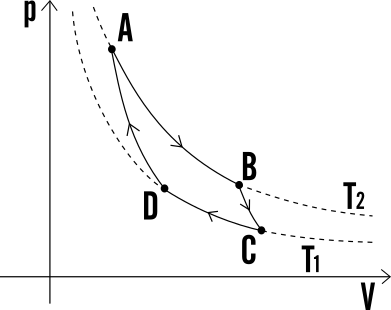
\includegraphics[scale=0.4]{ciclo-di-carnot}
    \centering
    \caption{Ciclo di Carnot}
\end{figure}

Nello stato \(A\) il gas è in equilibrio a contatto termico con una sorgente di calore a temperatura \(T_2\).
L'espansione isoterma reversibile \(AB\) può essere considerata come una successione di trasformazioni infinitesime: in ciascuna a seguito di una diminuzione \(dp\) della pressione esterna (equilibrio meccanico) il gas si espande di una quantità \(d V\) raffreddandosi di \(d T\); si ha quindi cessione di calore \(d Q\) dalla sorgente a temperatura \(T_2\) (equilibrio termico) al gas che ritorna alla temperatura \(T_2\). 
Come risultato, il gas passa in maniera reversibile dallo stato \(A\), di coordinate termodinamiche \(p_A\), \(V_A\), \(T_A\), allo stato \(B\) di coordinate \(p_B\), \(V_B\), \(T_B\), assorbendo il calore
\begin{equation*}
    Q_A = n R T_2 \ln \frac{V_B}{V_A} = W_{AB}
\end{equation*}
\(W_{AB}\) è il lavoro fatto dal gas nell'espansione isoterma. 

Nella trasformazione \(B C\) il gas è isolato da qualsiasi sorgente di calore. 
Seguendo lo schema adottato per la trasformazione \(AB\), durante ciascuna trasformazione infinitesima si ha una diminuzione \(d p\) della pressione esterna, un'espansione \(d V\) e un raffreddamento \(d T\). 
Il gas passa quindi dallo stato \(B\) (\(p_B, V_B, T_B\)) allo stato \(C\) ( \(p_C, V_C, T_1\) ), con \(T_1\) minore di \(T_2\) e, secondo \(TV^{\gamma-1} = costante\):
\begin{equation*}
    T_2 V_B^{\gamma - 1} = T_1 V_C^{\gamma-1}
\end{equation*}
Il lavoro fatto dal gas è \(W_{BC} = -\Delta U_{BC} = n c_V \left(T_1 - T_2\right)\).

Nella trasformazione \(C D\) il gas è a contatto termico con una sorgente di calore a temperatura \(T_1\). 
Il processo è analogo ad \(A B\), però ora si aumenta la pressione esterna di \(d p\), il gas si comprime di una quantità \(d V\) ed aumenta la sua temperatura di \(d T\), cede \(d Q\) alla sorgente a temperatura \(T_1\) e ritorna alla temperatura \(T_1\). 
Il calore ceduto complessivamente è 
\begin{equation*}
    Q_C = n R T \ln \frac{V_D}{V_C} = W_{CD}
\end{equation*}
ed è negativo, come il lavoro, poiché \(V_D < V_C\).

Infine nella trasformazione \(D A\) il gas è di nuovo isolato termicamente, si aumenta la pressione esterna di \(d p\), il volume del gas diminuisce di \(d V\) e  la temperatura aumenta di \(d T\). 
Il gas ritorna nello stato iniziale e vale, avendo assunto \(\gamma\) costante, la relazione
\begin{equation*}
    T_2 V_A^{\gamma - 1} = T_1 V_D^{\gamma - 1}
\end{equation*}
Il lavoro subito è \(W_{DA} = -\Delta U_{DA} = n c_V \left(T_1 - T_2\right) = - W_{BC}\)

Sommando tutti i contributi otteniamo
\begin{equation*}
    Q = Q_A + Q_C = W = W_{AB} + W_{BC} + W_{CD} + W_{DA} = W_{AB} + W_{CD}
\end{equation*}
questa quantità coincide con l'area racchiusa dal ciclo.

Il rendimento del ciclo è:
\begin{equation*}
    \eta = 1 + \frac{Q_C}{Q_B} = 1 + \frac{n R T_1 \ln \left(V_D / V_C \right) }{n R T_2 \ln \left(V_B / V_A \right)} = 1 - \frac{T_1 \ln \left(V_D / V_C \right) }{T_2 \ln \left(V_B / V_A \right)}
\end{equation*}

Dividendo membro a membro i termini delle relazioni
\begin{equation*}
    T_2 V_B^{\gamma - 1} = T_1 V_C^{\gamma - 1} \ , \ T_2 V_A^{\gamma - 1} = T_1 V_D^{\gamma - 1} 
\end{equation*}
ottenendo \(\left(\frac{V_B}{V_A}\right)^{\gamma - 1} = \left(\frac{V_C}{V_D}\right)^{\gamma - 1}\) ovvero \(\left(\frac{V_B}{V_A}\right) = \left(\frac{V_C}{V_D}\right)\).

Quindi
\begin{equation}
    \eta = 1 - \frac{T_1}{T_2}
\end{equation}

Si noti il fatto molto importante che non compare alcuna grandezza caratteristica del gas, ma solo i valori delle temperature delle sorgenti con cui il gas scambia calore: 
\emph{il rendimento del ciclo di Carnot, descritto da un gas ideale con calore specifico costante, dipende solo dalle temperature a cui avvengono gli scambi isotermi di calore}.

Poiché \(T_1 < T_2\) verifichiamo che \(\eta<1\); inoltre da \(V_B / V_A\) e \(Q_A > | Q_C | \). 
Il gas complessivamente assorbe calore perché \(Q_A + Q_C > 0\) e produce il lavoro \(W = Q_A + Q_C\), pari alla somma algebrica di quello fatto durante l'espansione isoterma e subito durante la compressione isoterma (i lavori svolti durante le adiabatiche sono eguali ed opposti). 

\subsection{Ciclo di Otto}

Il ciclo termico di Otto schematizza il funzionamento di un motore a scoppio a quattro tempi, come quello del motore automobilistico a benzina. 
Nel ciclo di Otto si suppone che la miscela aria-benzina sia assimilabile a un gas ideale biatomico e che il ciclo sia reversibile. 

\begin{figure}[h]
    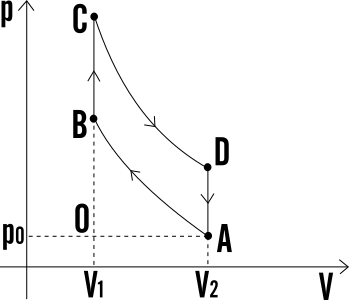
\includegraphics[scale=0.4]{ciclo-otto}
    \centering
    \caption{Ciclo di Otto}
\end{figure}

\begin{enumerate}
    \item Nella trasformazione \(O A\) la miscela benzina-aria viene aspirata nel cilindro, a pressione costante (\emph{fase di aspirazione}). 
    \item Nella trasformazione adiabatica reversibile \(A B\) la miscela nel cilindro viene compressa rapidamente dal pistone dal volume \(V_2\) al volume \(V_1\) (\emph{fase di compressione}). 
    \item La trasformazione \(B C\) schematizza l'incendio della miscela dovuto alla scintilla prodotta dalla candela con conseguente esplosione, che provoca una rapida crescita della temperatura e della pressione del gas; 
    si assume che il riscaldamento sia isocoro con assorbimento di calore da una successione di sorgenti a temperatura crescente
    \begin{equation*}
        Q_A = n c_V (T_C - T_B)
    \end{equation*}
    Questa è la fase di \emph{accensione e combustione}. 
    \item Il gas caldo si espande rapidamente spingendo il pistone e ritornando al volume \(V_2\) con una trasformazione adiabatica reversibile \(C D\), durante la quale viene compiuto lavoro (\emph{fase di espansione}). 
    \item La trasformazione \(D A\), isocora reversibile con la cessione del calore
    \begin{equation*}
        Q_C = n c_V ( T_A - T_D)
    \end{equation*}
    schematizza l'apertura della valvola verso il tubo di scappamento con conseguente riduzione della pressione al valore iniziale, mentre il gas cede calore all'ambiente (\emph{fase di decompressione}).
    \item Infine nella trasformazione \(A O\) a pressione costante il gas viene espulso dal cilindro e il pistone ritorna nella posizione iniziale (\emph{fase di scarico}). 
    I \emph{quattro tempi} sono le trasformazioni \( O A, AB, CD, A O\). 

    Il \emph{rendimento} del ciclo di Otto è dato da
    \begin{equation*}
        \eta = 1 + \frac{Q_C}{Q_A} = 1 - \frac{n c_V (T_A -T_D)}{n c_V (T_C - T_B)} = 1 + \frac{n c_V (T_D -T_A)}{n c_V (T_C - T_B)}
    \end{equation*}
    che idealmente corrisponde a circa \(0.6\) .
\end{enumerate}

Sperimentalmente è molto più facile misurare i volumi \(V_1 = V_B = V_C\) e \(V_2 = V_A = V_D\) e il loro rapporto \(r = V_2 / V_1\) (\emph{rapporto di compressione}). 
Dalle relazioni 
\begin{equation*}
    T_D V_2^{\gamma - 1} = T_C V_1^{\gamma - 1} \ , \ T_A V_2^{\gamma - 1} = T_B V_1^{\gamma - 1} 
\end{equation*}
sottraendo membro a membro si ottiene
\begin{equation*}
    \left(T_D - T_A\right) V_2^{\gamma - 1} = \left(T_C - T_B \right) V_1^{\gamma - 1}
\end{equation*}
Pertanto
\begin{equation*}
    \eta = 1 - (\frac{V_1}{V_2})^{\gamma - 1} = 1 - \frac{1}{r^{0.4}}
\end{equation*}
avendo utilizzato \(\gamma = 1.4\), valore valido per un gas biatomico.

Il rendimento aumenta all'aumentare del rapporto di compressione, che però non deve assumere valori troppo grandi se si vuole evitare il fenomeno dell'auto-combustione, cioè l'esplosione anticipata dovuta al riscaldamento della miscela durante la fase di compressione. 

Il rendimento del ciclo di Otto calcolato con la formula appena ricavata va inteso come valore massimo teorico: nei motori reali si ottengono rendimenti \(0.2 - 0.3\), contro \(0.6\) ideale. 
La differenza è dovuta a varie cause: innanzitutto il ciclo è solo un'approssimazione dei processi reali, che non possono essere così semplificati; per esempio le fasi di combustione ed espansione non sono nettamente separate, le fasi di compressione ed espansione sono state assunte adiabatiche perché molto rapide, cosicché sia trascurabile lo scambio di calore con l'esterno, ma non sono certamente reversibili (non c'è equilibrio meccanico). 
Inoltre sono stati trascurati gli attriti e le perdite di calore attraverso le pareti del cilindro. 
D'altra parte è importante avere un modello che indichi le massime prestazioni possibili.

\subsection{Ciclo frigorifero}

In un ciclo frigorifero il sistema complessivamente assorbe lavoro e cede calore (\(Q = W < 0\)). 
Nella situazione più semplice il sistema assorbe il calore \(Q_0\) dalla sorgente fredda, assorbe lavoro e cede il calore \(Q_C\) a una sorgente calda: risulta sempre \(|Q_C| > Q_0\).

Si definisce \emph{efficienza} o \emph{coefficiente di prestazione} di un ciclo frigorifero il rapporto
\begin{equation}
    \xi = \frac{Q_0}{W}
\end{equation}
tanto maggiore quanto minore è il modulo del lavoro speso nel ciclo, a parità di calore \(Q_0\) assorbito. 

\subsection{Ciclo di Carnot Inverso}

Un ciclo di Carnot percorso in senso inverso costituisce un esempio di ciclo frigorifero reversibile.
Il gas assorbe il calore $Q_0 = n R T_1 \ln (V_C / V_D )$ dalla sorgente alla temperatura $T_1$ (sorgente fredda) e cede il calore $Q_C = n R T_2 \ln (V_A / V_B )$ alla sorgente alla temperatura $T_2$ (sorgente calda), assorbendo il lavoro $W = Q_0 + Q_C$. 
L'efficienza è 
\begin{equation*}
    \xi = \frac{Q_0}{Q_C + Q_0} = \frac{n R T_1 \ln (V_C / V_D )}{n R T_2 \ln (V_B / V_A ) - n R T_1 \ln (V_C / V_D )} = \frac{T_1}{T_2 - T_1}
\end{equation*}
ricordando che \(V_B / V_A = V_C / V_D\).

Anche per i cicli frigoriferi sono verificati alcuni fatti di carattere generale: 
il calore ceduto dal sistema alle sorgenti calde è sempre maggiore, in modulo, di quello assorbito, cioè sottratto alla sorgente fredda e quindi il processo avviene sempre in presenza di lavoro fornito dall'ambiente al sistema ($Q_0 + |W| = | Q_C |$).

\section{Teoria cinetica dei gas}

\subsection{Modello cinetico del gas ideale}

\begin{enumerate}
    \item \emph{un gas è costituito da molecole uguali, in modo continuo e disordinato}
    \item \emph{gli urti tra molecole e tra molecole e parenti del contenitore sono elastici}
    \item \emph{non ci sono forze intermolecolari, se non durante gli urti}: gli urti sono dovuti cioè a forze repulsive a corto raggio di azione, mentre si assumono trascurabili le forze attrattive tra le molecole
    \item \emph{le dimensioni delle molecole sono molto piccole rispetto alle distanze medie tra di esse}
\end{enumerate}

Sulla base della prima ipotesi (caos molecolare), in ogni istante, considerata una qualsiasi direzione orientata \(\overrightarrow{u}\), ci sono tante molecole che hanno velocità concorde a \(\overrightarrow{u}\) quante hanno velocità discorde a \(\overrightarrow{u}\); la velocità media \(\overrightarrow{v}_m\) è quindi nulla. 
Infatti macroscopicamente un gas chiuso in un recipiente è in quiete, \(\overrightarrow{P} = M \overrightarrow{v}_{CM}\). 
Inoltre il numero di molecole per unità di volume deve essere lo stesso in ogni parte del recipiente occupato dal gas (densità costante).

La seconda ipotesi implica che negli urti tra molecole si conservano quantità di moto ed energia, mentre nell'urto di una molecola contro una parete si conserva solo l'energia (forze esterne impulsive)

Dalla terza ipotesi deriva che l'energia potenziale interna è nulla e quindi la sola forma di energia è quella cinetica.

Infine la quarta ipotesi indica che il volume totale occupato dalle molecole è trascurabile rispetto a quello del recipiente.

Sulla base di questo modello cinetico è stata sviluppata la teoria cinetica dei gas, che permette di arrivare a previsioni sul comportamento dei gas, che si possono verificare sperimentalmente.

\subsection{Calcolo della pressione}

Si considera un contenitore cubico di lato \(a\) riempito con un gas che si comporta come prescritto dal modello cinetico. 
La velocità di una molecola è data da \(\overrightarrow{v} = v_x \overrightarrow{u_x} + v_y \overrightarrow{u_y} + v_z \overrightarrow{u_z}\) con le componenti alle pareti opposte.

Nell'urto elastico contro la parete \(y z\) cambia solo la componente \(v_x \overrightarrow{u}_x\) che diventa \(-v_x \overrightarrow{u}_x\) mentre le altre rimangono invariate, data l'assenza di forze di attrito.
La variazione di quantità di moto nell'urto della molecola con la parete \(y z\) è pari a \(-2 m v \overrightarrow{u}_x\), se \(m\) è la massa della molecola, e quindi l'impulso comunicato alla parete è \(2 m v_x \overrightarrow{u}_x\).

L'urto successivo contro la parete \(y\): considerata avviene dopo un tempo \(t = 2a / v\), necessario per attraversare nei due sensi il cubo lungo la direzione \(x\). 
In realtà non è la stessa molecola che compie l'urto successivo perché nel tragitto \(2a\) essa può subire un urto contro un'altra molecola e venire deviata. 
Tuttavia, a causa del moto completamente disordinato (prima ipotesi), per una molecola che perde la componente \(v_x\), ce n'è un'altra che, a seguito di un urto, acquista tale componente \(v_x\). 

Pertanto il numero di urti al secondo sulla parete \(y z\) è dato da \(\frac{1}{t} = \frac{v_c}{2a}\) e l'impulso comunicato in un secondo, pari alla componente \(x\) della forza media esercitata sulla parete da una molecola, vale in modulo:
\begin{equation*}
    F_x = 2m v_x \frac{v^2_x}{2a} = \frac{m v^2_x}{a}
\end{equation*}

La forza risultante sulla parete è
\begin{equation*}
    R_x = \frac{m}{a} \sum_i v_{x,i}^2
\end{equation*}
dove la somma è estesa a tutte le molecole; la pressione sulla parete \(y z\) di area \(S = a^2\), dovuta agli urti molecolari, risulta essere quindi

\begin{equation*}
    p = \frac{R_x}{S} = \frac{m}{a^3} \sum_i v_{x,i}^2 = \frac{N m}{V} \frac{1}{N} \sum_i v_{x,i}^2
\end{equation*}
dove \(N\) è il numero totale di molecole nel cubo di volume \(V= a^3\). 

Si chiama velocità media quadratica la quantità \(\bar{v}\), definita come radice quadrata di 
\begin{equation*}
    \bar{v}^2 =  \bar{v}^2_x + \bar{v}^2_y + \bar{v}^2_z = \frac{1}{N} \sum_i \left(v_{x,i}^2 + v_{y,i}^2 + v_{z,i}^2\right)
\end{equation*}
Se il moto è completamente disordinato non c'è alcuna direzione preferita per le molecole e pertanto i valori medi quadratici \(\bar{v}_x^2, \bar{v}_y^2, \bar{v}_z^2\) sono eguali tra loro:
\begin{equation*}
    \bar{v}_x^2 = \bar{v}_y^2 = \bar{v}_z^2 = \frac{\bar{v}^2}{3}
\end{equation*}

In conclusione
\begin{equation*}
    p = \frac{N m}{V} \frac{\bar{v}^2}{3} \implies pV = \frac{1}{3} N m \bar{v}^2
\end{equation*}

Il ragionamento è identico per quanto riguarda gli urti sulle altre pareti e si estende a contenitori di forma qualunque. 
Il risultato è generale, nel senso che non dipende da come sono distribuite le velocità delle singole molecole in un gas alla temperatura \(T\), finché tutte le direzioni del moto sono equivalenti. 

Definendo come energia cinetica media di traslazione delle molecole \(\bar{E_k} = \frac{1}{2} m \bar{v}^2\), si ha 
\begin{equation*}
    p V = \frac{2}{3} N \bar{E_k}
\end{equation*}
\emph{il prodotto pressione per volume è proporzionale all'energia cinetica media delle molecole N\(\bar{E_k}\), che nel gas ideale coincide con l'energia totale}.

Per un gas ideale ho che \(p V = n R T\); eguagliando si trova:
\begin{equation*}
    \bar{E_k} = \frac{3}{2} \frac{n}{N} R T = \frac{3}{2} \frac{R}{N_A} T
\end{equation*}
dato che \(n N_A = N\).

\begin{equation}
    \bar{E_k} = \frac{3}{2} k_B T
\end{equation}
\emph{l'energia cinetica media di una molecola di un gas ideale è proporzionale alla temperatura del gas.}
Abbiamo trovato il significato microscopico della grandezza temperatura: \emph{essa è proporzionale all'energia cinetica media delle molecole}. 

\subsection{Equipartizione dell'energia}
Lo sviluppo successivo della teoria cinetica dei gas porta alla previsione che la relazione precedente è di carattere generale, in questo senso: 
ad ogni termine quadratico dell'energia classica di una molecola di un corpo corrisponde, all'equilibrio termodinamico, un'energia media pari a \(\frac{1}{2} k_B T\), essendo \(T\) la temperatura del sistema. 
Questo risultato può essere anche espresso affermando che ad ogni componente indipendente del moto compete la stessa energia media \emph{ossia per ogni grado di libertà c'è il contributo} \(\frac{1}{2} k_B T\); 
esso è noto come \emph{principio dell'equipartizione dell'energia}. 

Pertanto per un sistema con \(l\) gradi di libertà
\begin{equation}
    \bar{E} = \frac{l}{2} k_B T
\end{equation}

Le molecole di un gas ideale monoatomico presentano \emph{tre gradi di libertà} e la loro energia, esclusivamente cinetica, ha tre termini quadratici:
\begin{equation*}
    E_k = \frac{1}{2} m v_x^2 + \frac{1}{2} m v_y^2 + \frac{1}{2} m v_z^2
\end{equation*}
Per esse il principio dell'equipartizione dell'energia prevede 
\begin{equation*}
    \bar{E_k} = \bar{E}_x + \bar{E}_y + \bar{E}_z = \frac{3}{2} k_B T
\end{equation*}

Le energie cinetiche medie calcolate per le molecole monoatomiche e biatomiche sono l'unica forma di energia interna di un gas e allora, per una mole di gas, deve sussistere l'eguaglianza:
\begin{equation*}
    \Delta U = c_V \Delta T = \Delta E_k = \frac{l}{2} N_A k_B \Delta T = \frac{l}{2} R \Delta T
\end{equation*}
da cui ricavo il calore specifico molare a volume costante
\begin{equation*}
    c_V = \frac{l}{2} R
\end{equation*}

Pertanto per le molecole monoatomiche che hanno \(l = 3\)
\begin{equation*}
    c_V = \frac{3}{2} R
\end{equation*}
per le molecole biatomiche con \(l = 5\)
\begin{equation*}
    c_V = \frac{5}{2} R
\end{equation*}
\end{document}